\documentclass[10pt,a4paper]{article}
\usepackage[utf8]{inputenc}
\usepackage[T1]{fontenc}
\usepackage{lmodern}
\usepackage[margin=2.3cm]{geometry}
\usepackage{booktabs,graphicx,amsmath,amssymb,array,caption,enumitem,xcolor}
\usepackage{float}
\usepackage[hidelinks]{hyperref}
\sloppy\emergencystretch=4em
\captionsetup{font=small,labelfont=bf,justification=justified,singlelinecheck=false}
\setlength{\parindent}{0pt}\setlength{\parskip}{5pt}
\newcommand{\kalla}[1]{\par\noindent\textbf{Källa:} #1\par}
\newcommand{\raknas}{\par\noindent\textbf{Så räknas den.} }
\newcommand{\visar}{\par\noindent\textbf{Vad den visar.} }
\newcommand{\kod}[1]{\texttt{#1}}
\newcommand{\BD}{Ben-David m.fl.\ (2022)}
\newcommand{\ACF}{Adelino m.fl.\ (2017)}
\begin{document}

\begin{center}
{\Large\bfseries Slutligt underlag: tabeller, figurer och formler}\\[3pt]
{\large BE451, Alexander Fox och Ludvig Pauli Uväng}\\[3pt]
Byggt 21 november 2026 med \kod{final\_code/kor\_allt.sh}
\end{center}

\section*{Läs detta först}
\begin{itemize}[leftmargin=*,itemsep=1pt]
\item Dokumentet samlar det som kan stå i uppsatsen: sex tabeller, fyra figurer och bilaga A1 till A7. Efter varje tabell står hur den är räknad, formeln och källan.
\item \textbf{Inget eget test finns med.} Varje test är ankarets (Ben-David m.fl.\ 2022) eller Adelino m.fl.\ (2017), ur artikeln eller författarnas kod. Det som ändå saknar förlaga står samlat i avsnittet ``Kvar utan förlaga''.
\item Alla tal är körda av AI (Claude). Ingen av författarna har kört om något. Tabellerna skrivs av koden ur \kod{final\_result/tal/}; inga tal är inskrivna för hand utom ankarets egna.
\item Tabeller, figurer och tabelltexter är på engelska så att de kan lyftas in. Förklaringarna är på svenska.
\item Där ankarets kod och tryckta text skiljer sig följer vi koden (beslut 20 november); skillnaderna står i avsnitt~\ref{sec:avvik}.
\end{itemize}

\section*{Struket 20 november: egna test}
\begin{itemize}[leftmargin=*,itemsep=1pt]
\item Betyg $\times$ Efter $\times$ Äldre för 2006 (tidigare tabell 3, panel C), i alla tre varianter.
\item Samma fonder före och efter 2006.
\item Uppdelningen på fondens ålder i testen av 2006, och kravet på minst 200 fonder för jämförelseår.
\item ``Sicksacken'' (polynom i volatilitet och flöde före bytet), låtsasbytet januari 2021, fem och tjugo volatilitetsgrupper, inplanterad effekt.
\item Risksiffran inom kategori och uppdelad på perioderna före och efter 2023.
\item Betyget mätt vid slutet av månad $t-1$.
\item Testen i Reuter och Zitzewitz form.
\end{itemize}

\section*{Ändrat mot tidigare rapporterade tal}
\begin{enumerate}[leftmargin=*,itemsep=1pt]
\item \textbf{Ankarets tabell 2 (bilaga A2) var fel uppställd.} Kolumn 2 till 5 har rå avkastning och ett mått till i samma regression. Tidigare kördes en regression per mått. Rättat.
\item \textbf{Figur 3.} Det kommande betyget hämtas ur urvalet i händelsemånaden, som i koden.
\item \textbf{Tabell 3, panel B.} Andelen räknas över alla fondmånader mot fondens föregående rad, som i koden.
\item \textbf{Tabell 5.} Observationer som är ensamma i sin grupp tas bort, som \kod{reghdfe} gör: 0,0038 före (var 0,0040).
\item \textbf{Tabell 6.} Flödet winsoriseras vid 1/99 som hos ankaret (var 2,5/97,5), och standardfelen klustras på fond som hos Adelino m.fl.\ (var det större av två). Huvudtalet är $+0{,}01$ (0,82) (var $+0{,}07$ (0,69)); stjärnan 5,99 (var 5,29).
\item \textbf{Femårskravet infört i alla urval (21 november).} Barber, Huang och Odean kräver fem års avkastningshistorik för att en fond ska ingå; vi krävde 36 månader. \textbf{Alla tal för USA och Europa utom tabell 6 är därför nya.} USA: 193~059 fondmånader (var 233~290); stjärnan mot rå avkastning 0,217 (var 0,280). Europa: urvalet börjar juni 2019 (var januari 2018), 94~203 fondmånader (var 130~031); risksiffran som tredje signal $+1{,}08$ (var $+0{,}61$), fortfarande inte skild från noll. Europa 2006: urvalet börjar juni 2004 (var januari 2003), 24~924 fondmånader före bytet (var 57~043); händelsetestet ligger nu över gränsen i båda måtten. Jämförelsen före och efter står i avsnittet om urvalet.
\end{enumerate}

\section{Källor till formler och metoder}\label{sec:kallor}
\begin{description}[leftmargin=1.6cm,style=nextline,itemsep=2pt]
\item[{[BD]}] Ben-David, I., J. Li, A. Rossi och Y. Song (2022). What Do Mutual Fund Investors Really Care About? \textit{Review of Financial Studies} 35(4), 1723--1774. Tryckt version, läst i sin helhet. Sidnummer nedan avser trycket.
\item[{[BD-kod]}] Författarnas kod till [BD] (SAS och Stata), filen \kod{11.docx}. Hänvisningar anger kodens egna rubriker.
\item[{[ACF]}] Adelino, M., I. Cunha och M. A. Ferreira (2017). The Economic Effects of Public Financing: Evidence from Municipal Bond Ratings Recalibration. \textit{Review of Financial Studies} 30(9), 3223--3268. Tryckt version. Lästa av Claude i denna körning: s.~3236--3237 och 3242--3245 (ekvation~1, tabell 3 och 5, figur 4). Hela artikeln är läst i arbetsversion av en annan session (\kod{NOTIS\_sex\_artiklar\_lasta\_i\_sin\_helhet\_2026-11-20}).
\item[{[BHO]}] Barber, B. M., X. Huang och T. Odean (2016). Which Factors Matter to Investors? Evidence from Mutual Fund Flows. \textit{Review of Financial Studies} 29(10), 2600--2642. Läst 21 november i SSRN-versionen daterad 18 maj 2016 (brödtext, tabell 1, tabellnoter, nätbilagans metoddel). \textbf{Den tryckta versionen är inte läst.} Hänvisningar avser avsnitt och noter i SSRN-versionen.
\item[{[FM]}] Fama, E. F. och J. D. MacBeth (1973). Risk, Return, and Equilibrium: Empirical Tests. \textit{Journal of Political Economy} 81(3), 607--636. \textbf{Inte läst.} Metoden används så som [BD] beskriver den (bilaga B.3, s.~1767; tabell 6, s.~1761).
\item[{[CGM]}] Cameron, A. C., J. B. Gelbach och D. L. Miller (2011). Robust Inference with Multiway Clustering. \textit{Journal of Business \& Economic Statistics} 29(2), 238--249. \textbf{Inte läst.} Formeln är den som Statas \kod{reghdfe} använder i [BD-kod].
\item[{[MS]}] Morningstar (2023). The Morningstar Rating for Funds. Morningstar Methodology, april 2023, 20 sidor. \url{https://s25.q4cdn.com/634000362/files/doc_downloads/1/1157231.pdf}. Bilaga 2 (s.~19) och exhibit 5 (s.~15) kontrollerade 21 november. Hela dokumentet läst av en annan session (\kod{NOTIS\_kalla\_for\_morningstars\_metodbyte\_i\_europa\_oktober\_2006\_2026-11-20}).
\end{description}

\section{Data}
Alla filer ligger under \kod{data/riskklass\_2026-11/morningstar\_direct/} i repot. Datan är licensierad (Morningstar Direct, LSEG); repot ska vara privat.

{\small\begin{tabular}{@{}p{2.6cm}p{7.2cm}p{5.6cm}@{}}
\toprule
Urval & Fil & Innehåll \\
\midrule
USA 1991--2011 & \kod{exporter\_2026-11-18/} \kod{BA37C8D4\ldots csv.gz} & Morningstar Direct: amerikanska aktiefonder, avkastning, förmögenhet per andelsklass, betyg \\
Europa 2013--2025 & \kod{bas\_eu\_2026-11-19/A1, A2, A3, B1, B2} & Morningstar Direct: andelsklasser i Luxemburg och Irland, levande och nedlagda, med risksiffra (SRRI-historik, SRI) \\
Europa 1998--2016 & \kod{eu2006\_lseg\_bank\_2026-11-20/} \kod{radata/} & Morningstar Direct (två exporter) och fondförmögenhet ur LSEG 2002--2008 \\
Faktorer & \kod{faktorer/}, \kod{analys\_usa\_2026-11-18/} & Kenneth Frenchs datasamling: USA, Developed, Europe \\
\bottomrule
\end{tabular}}

\begin{table}[H]
\caption{Summary statistics. Fund-month observations. Flow is the monthly net flow in percent of the fund's assets a month earlier. The return measures are 18-month exponentially weighted averages of monthly excess returns and alphas, in percent per month. CS SD is the average of the monthly cross-sectional standard deviations (Panel D: the pooled standard deviation). The last three columns give the values in Table 1 of Ben-David et al.\ (2022).}
\centering\resizebox{\textwidth}{!}{\begin{tabular}{lrrrrrrrrrrr}
\toprule
 & $N$ & Mean & CS SD & P5 & P25 & P50 & P75 & P95 & \multicolumn{3}{c}{Ben-David et al.} \\
 & & & & & & & & & Mean & CS SD & P50 \\
\midrule
\multicolumn{12}{l}{\textit{Panel A. United States, July 1997 to December 2011 (233,290 fund-months, 2,638 funds; Ben-David et al.: 248,463 and 3,341)}} \\
Fund size (USD million) & 233,290 & 1,297.79 & 3,165.29 & 20.88 & 95.43 & 307.37 & 1,007.84 & 5,869.11 & 1,472.00 & 3,038.00 & 411.00 \\
Age (years) & 233,290 & 15.29 & 12.96 & 5.00 & 7.44 & 11.18 & 17.27 & 42.38 & 16.90 & 12.80 & 12.80 \\
Flow (\%) & 233,290 & $-$0.21 & 3.81 & $-$4.91 & $-$1.54 & $-$0.47 & 0.72 & 5.60 & $-$0.54 & 2.18 & $-$0.61 \\
Flow (USD million) & 233,290 & $-$1.41 & 44.18 & $-$49.58 & $-$5.89 & $-$0.69 & 1.74 & 46.01 & $-$2.60 & 52.40 & $-$1.20 \\
Raw excess return (\%) & 233,290 & 0.33 & 0.83 & $-$3.78 & $-$0.55 & 0.66 & 1.61 & 2.97 & 0.34 & 0.99 & 0.71 \\
Market-adjusted (\%) & 233,290 & 0.03 & 0.83 & $-$1.30 & $-$0.42 & $-$0.03 & 0.43 & 1.51 & 0.07 & 0.99 & 0.01 \\
CAPM alpha (\%) & 233,290 & 0.05 & 0.78 & $-$1.20 & $-$0.38 & $-$0.00 & 0.43 & 1.43 & 0.09 & 0.95 & 0.03 \\
FF3 alpha (\%) & 233,290 & $-$0.08 & 0.59 & $-$1.04 & $-$0.41 & $-$0.10 & 0.21 & 0.90 & $-$0.03 & 0.78 & $-$0.07 \\
FFC alpha (\%) & 233,290 & $-$0.08 & 0.54 & $-$0.98 & $-$0.39 & $-$0.09 & 0.20 & 0.82 & $-$0.03 & 0.76 & $-$0.06 \\
\addlinespace
\multicolumn{12}{l}{\textit{Panel B. Europe, January 2018 to December 2025 (130,031 fund-months, 2,307 funds)}} \\
Fund size (USD million) & 130,031 & 287.94 & 440.94 & 14.97 & 42.19 & 114.73 & 318.46 & 1,170.10 & & & \\
Age (years) & 130,031 & 13.37 & 6.90 & 4.61 & 7.36 & 12.19 & 18.50 & 25.66 & & & \\
Flow (\%) & 130,031 & $-$0.49 & 5.24 & $-$7.38 & $-$1.53 & $-$0.29 & 0.58 & 6.06 & & & \\
Flow (USD million) & 130,031 & $-$0.63 & 14.41 & $-$18.68 & $-$1.97 & $-$0.19 & 0.61 & 16.28 & & & \\
Raw excess return (\%) & 130,031 & 0.46 & 0.91 & $-$2.49 & $-$0.45 & 0.56 & 1.47 & 3.02 & & & \\
Market-adjusted (\%) & 130,031 & $-$0.35 & 0.91 & $-$1.98 & $-$0.88 & $-$0.33 & 0.18 & 1.24 & & & \\
CAPM alpha (\%) & 130,031 & $-$0.35 & 0.88 & $-$1.94 & $-$0.86 & $-$0.33 & 0.17 & 1.18 & & & \\
FF3 alpha (\%) & 130,031 & $-$0.24 & 0.79 & $-$1.60 & $-$0.71 & $-$0.25 & 0.20 & 1.19 & & & \\
FFC alpha (\%) & 130,031 & $-$0.28 & 0.80 & $-$1.70 & $-$0.75 & $-$0.28 & 0.16 & 1.14 & & & \\
Star rating & 130,031 & 3.05 & 1.08 & 1.00 & 2.00 & 3.00 & 4.00 & 5.00 & & & \\
Risk number & 118,102 & 5.18 & 0.57 & 4.00 & 4.00 & 5.00 & 6.00 & 6.00 & & & \\
\addlinespace
\multicolumn{12}{l}{\textit{Panel C. Europe, January 2003 to December 2010 (161,065 fund-months)}} \\
Fund size (USD million) & 161,065 & 315.77 & 557.13 & 14.28 & 37.73 & 100.06 & 292.58 & 1,419.87 & & & \\
Age (years) & 161,065 & 9.30 & 5.06 & 3.39 & 5.47 & 8.16 & 11.91 & 18.91 & & & \\
Flow (\%) & 161,065 & $-$0.21 & 7.66 & $-$10.61 & $-$2.54 & $-$0.45 & 1.39 & 11.45 & & & \\
Raw excess return (\%) & 161,065 & 0.58 & 1.06 & $-$5.28 & $-$0.16 & 1.03 & 2.11 & 3.81 & & & \\
Star rating & 161,065 & 2.96 & 1.09 & 1.00 & 2.00 & 3.00 & 4.00 & 5.00 & & & \\
\addlinespace
\multicolumn{12}{l}{\textit{Panel D. The January 2023 switch, January 2021 to December 2024 (230,531 fund-months, 4,818 funds; the number fell 0, 1, 2 classes for 418, 2,574, 1,826 funds)}} \\
Flow (\% per month) & 230,531 & $-$0.29 & 4.71 & $-$6.47 & $-$1.53 & $-$0.28 & 0.67 & 6.27 & & & \\
Star rating & 197,296 & 3.16 & 1.05 & 1.00 & 2.00 & 3.00 & 4.00 & 5.00 & & & \\
Volatility (\%, per fund) & 4,818 & 12.57 & 6.77 & 2.76 & 6.96 & 11.82 & 17.83 & 23.23 & & & \\
Classes the number fell (per fund) & 4,818 & 1.29 & 0.62 & 0.00 & 1.00 & 1.00 & 2.00 & 2.00 & & & \\
Assets Dec 2022 (USD million, per fund) & 4,816 & 538.08 & 1,523.54 & 8.15 & 42.26 & 142.38 & 443.59 & 2,198.40 & & & \\
\bottomrule
\end{tabular}
}
\end{table}
\raknas Medel, percentiler och spridning på fondmånader efter alla urvalssteg. CS SD är medelvärdet av månadens standardavvikelse över fonder.
\kalla{[BD] tabell 1, s.~1734; [BD-kod] ``Code and Output for: Table 1. Sample Summary Statistics''. Kod: \kod{lib/ankartest.py:table1}.}

\section{Variabler och formler}\label{sec:var}
\textbf{Flöde.} För andelsklass $c$ i månad $t$, med förmögenhet $NA$ och avkastning $R$:
\begin{equation}
\text{DF}_{c,t}=NA_{c,t}-NA_{c,t-1}(1+R_{c,t}),\qquad
F_{p,t}=100\cdot\frac{\sum_{c\in p}\text{DF}_{c,t}}{\sum_{c\in p}NA_{c,t-1}} .
\end{equation}
Summan går över fondens klasser med förmögenhet båda månaderna. Exempel: 100 MUSD förra månaden, 5~\% avkastning och 110 MUSD nu ger $\text{DF}=110-105=5$ och $F=5~\%$.
\kalla{[BD] ekvation 1, s.~1733: $F_{p,t}=TNA_{p,t}/TNA_{p,t-1}-(1+R_{p,t})$. Andelsklasser läggs ihop till fond eftersom de äger samma portfölj ([BD] s.~1732).}

\textbf{Urval.} Fonden ska ha minst 10 MUSD månaden före. Indexfonder ingår inte. Alla variabler winsoriseras vid 1:a och 99:e percentilen inom varje månad.
\kalla{[BD] s.~1733.}

\textbf{Betyg.} Fondens betyg är det förmögenhetsvägda medelvärdet av klassernas Morningstar Rating Overall, avrundat till heltal 1--5. Betyget mäts vid slutet av månad $t$, som i [BD-kod].

\textbf{Avkastningssignaler.} Betor skattas varje månad på de 60 föregående månaderna (minst 36 observationer). Månadens alfa är överavkastningen minus beta gånger faktoravkastningen. Signalen är ett vägt medel över de 18 föregående månaderna:
\begin{equation}
\text{ALPHA}_{p,t}=\frac{\sum_{s=1}^{18}e^{-\lambda(s-1)}\,\alpha_{p,t-s}}{\sum_{s=1}^{18}e^{-\lambda(s-1)}},\qquad \lambda=0{,}20551497 .
\end{equation}
Fem mått: rå överavkastning (utan faktorer), marknadsjusterad, CAPM, Fama-French tre faktorer (FF3) och Carhart fyra faktorer (FFC).
\kalla{[BD] s.~1733 och bilaga A.2, s.~1764--1765 (ekvation A.2 och A.3, vikterna och $\lambda$ på s.~1765); [BD-kod] ``INITIAL STEP: SETUP PRIMARY DATASET'' (\kod{\%let n\_years = 5}, \kod{\%let min\_mm = 36}, \kod{\%let Lambda = 0.20551497}, ``Apply BHO-style weighting of past returns''). Vikterna kommer ur [BHO] ekvation 5 enligt [BD]. Kod: \kod{bygg/usa\_panel.py}, \kod{bygg/eu\_5\_fondpanel.py}.}

\textbf{Standardfel.} Klustrade på fond och månad: $V=V_{\text{fond}}+V_{\text{månad}}-V_{\text{fond}\times\text{månad}}$.
\kalla{[BD] tabell 3, not, s.~1744 (``clustered by fund and month''); [BD-kod] \kod{vce(cluster yyyymm fundid2)}; formeln i [CGM]. Kod: \kod{lib/stat.py:ols}.}

\section{Följer flödena stjärnan?}
\begin{table}[H]
\caption{Flows, star ratings and past returns. Panel A follows Table 3 of Ben-David et al.\ (2022). Each month the funds with five stars are compared with an equal number of top funds by each return measure. The coefficient is $b_1$ in a regression of monthly flow (percent of assets) on the difference between the two top-fund indicators and an indicator for being top-ranked by either; it equals half the difference in flow between funds that only the first and only the second measure rank at the top. $t$-statistics, in parentheses, use standard errors clustered by fund and month. Panel B follows their Figure 3: the $R^2$ of a regression of flow on month effects, the 18-month raw return and star-rating indicators, minus the $R^2$ without the block named. Samples: United States July 1997 to December 2011; Europe June 2019 to December 2025.}
\centering\begin{tabular}{lcccccc}
\toprule
 & \multicolumn{2}{c}{Ben-David et al.} & \multicolumn{2}{c}{United States, ours} & \multicolumn{2}{c}{Europe, ours} \\
 & Coef. & $t$ & Coef. & $t$ & Coef. & $t$ \\
\midrule
\multicolumn{7}{l}{\textit{Panel A. Flow to top-ranked funds, pairwise (percent of assets per month)}} \\
Star rating vs Raw & 0.099 & (2.50) & 0.217 & (3.26) & $-$0.081 & ($-$0.88) \\
Star rating vs CAPM & 0.108 & (2.72) & 0.181 & (2.80) & $-$0.100 & ($-$1.12) \\
Star rating vs FF3 & 0.192 & (4.85) & 0.327 & (5.09) & 0.042 & (0.52) \\
Star rating vs FFC & 0.188 & (4.73) & 0.303 & (4.85) & 0.075 & (0.91) \\
Raw vs CAPM & 0.032 & (0.62) & $-$0.107 & ($-$1.17) & $-$0.085 & ($-$0.56) \\
Raw vs FF3 & 0.207 & (4.74) & 0.185 & (2.65) & 0.258 & (2.33) \\
\addlinespace
\multicolumn{7}{l}{\textit{Panel B. Share of flow variation explained beyond the other block (percent, equal-weighted)}} \\
Star rating & \multicolumn{2}{c}{6.5} & \multicolumn{2}{c}{5.1} & \multicolumn{2}{c}{0.5} \\
Past return & \multicolumn{2}{c}{5.6} & \multicolumn{2}{c}{2.5} & \multicolumn{2}{c}{1.2} \\
Fund-months & \multicolumn{2}{c}{248,463} & \multicolumn{2}{c}{193,059} & \multicolumn{2}{c}{94,203} \\
\bottomrule
\end{tabular}

\end{table}
\raknas Panel A. $\text{Top}^A_{p,t}=1$ om fonden har fem stjärnor (eller hör till de $n_t$ bästa på mått $A$, där $n_t$ är antalet femstjärniga fonder den månaden).
\begin{equation}
F_{p,t}=a+b_1\big(\text{Top}^A_{p,t}-\text{Top}^B_{p,t}\big)+b_2\max\big(\text{Top}^A_{p,t},\text{Top}^B_{p,t}\big)+e_{p,t}.
\end{equation}
Ingen månadseffekt. Den andra regressorn definieras inte i den kod vi har (variabeln heter \kod{morn5\_e\_unad5}); vi läser den som ``toppklassad av någon av de två''. Valet påverkar inte $b_1$: de två toppgrupperna är lika stora varje månad, så skillnaden är okorrelerad med varje symmetrisk regressor (bilaga A4, andra tabellen). Ankarets tryckta tal är kodens $b_1$ (0,099 i trycket, 0,0009926 i kodens utskrift). Panel B: $R^2_{\text{marg}}(\text{block})=R^2(\text{allt})-R^2(\text{allt utom blocket})$.
\kalla{Panel A: [BD] tabell 3, s.~1744, och figur 4, s.~1743 (lika många toppfonder som femstjärniga); [BD-kod] ``Table 3 (Flows to Top-Ranked Funds: Horse Races Between Performance Measures)'', raden \kod{reghdfe std\_floww morn\_gro5\_m\_unad\_gro5 morn5\_e\_unad5, noa vce(cluster yyyymm fundid2)}. Panel B: [BD] figur 3, s.~1741; [BD-kod] ``R\textasciicircum 2 regressions for Figure 3''. Kod: \kod{lib/ankartest.py:table3, fig3}.}
\visar I USA slår stjärnan varje avkastningsmått, som hos ankaret men med större koefficienter. I Europa går stjärnan inte att skilja från rå avkastning eller CAPM. Alla tio par står i bilaga A1.

\setcounter{figure}{1}
\begin{figure}[H]
\centering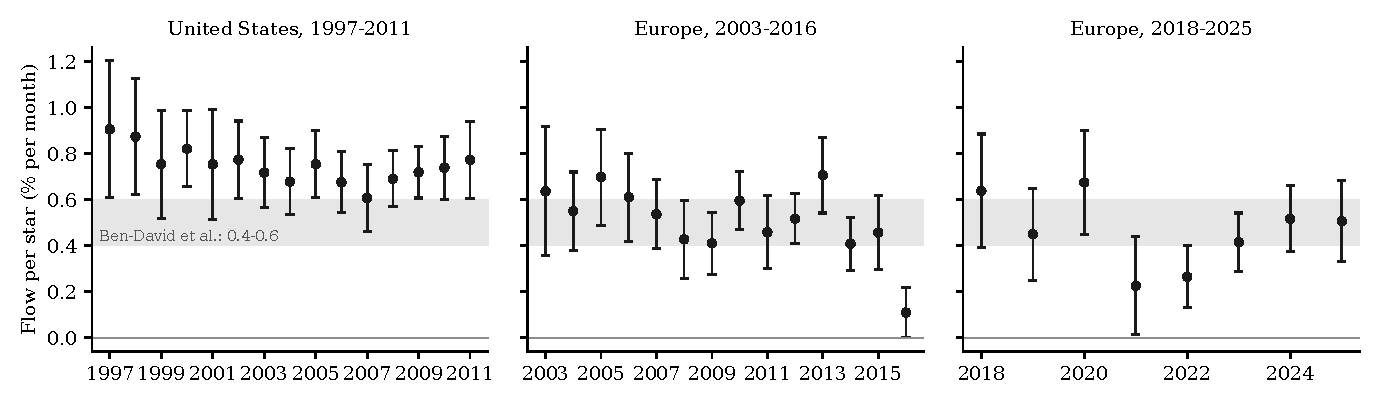
\includegraphics[width=\textwidth]{figurer/figur2.pdf}
\caption{Flow per star by year. Each point is the coefficient on the star rating (1 to 5) in a regression of monthly flow (percent of assets) on the rating, the 18-month raw return and controls, with month effects, estimated year by year; bars are 95 percent intervals with standard errors clustered by fund and month. The shaded band is the range Ben-David et al.\ (2022) report for the United States (0.4 to 0.6 percent, p.~1748). Controls in the first and third panel: flow 19 months earlier, log size, log age, expense ratio, 60-month return volatility. The middle panel has the raw return as its only control.}
\end{figure}
\raknas För varje kalenderår: $F_{p,t}=b\cdot\text{Betyg}_{p,t}+c\cdot\text{ALPHA}^{\text{rå}}_{p,t}+\gamma'X_{p,t}+\mu_t+e_{p,t}$.
\kalla{[BD] figur 5, panel A(b), s.~1747; [BD-kod] ``Regression for Panel A(b) of Figure 5'': \kod{reghdfe std\_floww100 rating retrf\_a lag19\_stdflow\_w99 lglagmtnaw\_w99 lgagew\_w99 portexpw\_w99 std\_ret\_60m\_w99 if yyyy == \ldots, a(yyyymm) vce(cluster fundid yyyymm)}. Kod: \kod{lib/ankartest.py:fig5a}.}

\textbf{Samma regression i två perioder.} Figuren visar ett tal per år. Tabellen nedan skattar samma regression före och efter reformen och ger skillnaden med standardfel:
\begin{equation}
F_{p,t}=b\,\text{Betyg}_{p,t}+d\,\text{Betyg}_{p,t}\times\text{Efter}_t+\gamma'X_{p,t}+\delta'X_{p,t}\times\text{Efter}_t+\mu_t+e_{p,t}.
\end{equation}
$\text{Efter}_t=1$ månaderna efter händelsemånaden, annars 0. $X$ är rå avkastning och kontrollerna i figuren. $b$ är flödet per stjärna före, $b+d$ efter, och $d$ skillnaden, i procent av förmögenheten per månad. Standardfel i parentes, klustrade på fond och månad.
\begin{center}\resizebox{0.95\textwidth}{!}{\begin{tabular}{lcccccc}
\toprule
 & Before & After & Difference & $t$ & Fund-months before & Fund-months after \\
\midrule
United States, June 2002 (1997--2011) & 0.804 (0.061) & 0.677 (0.029) & $-$0.128 (0.065) & $-$1.96 & 40,250 & 150,105 \\
Europe, October 2006 (to 2016) & 0.590 (0.089) & 0.401 (0.030) & $-$0.190 (0.093) & $-$2.04 & 24,924 & 192,690 \\
Europe, October 2006 (to 2015) & 0.590 (0.089) & 0.435 (0.031) & $-$0.156 (0.093) & $-$1.67 & 24,924 & 173,298 \\
Europe, October 2006 (to 2010) & 0.590 (0.089) & 0.390 (0.046) & $-$0.201 (0.099) & $-$2.03 & 24,924 & 73,592 \\
\bottomrule
\end{tabular}
}\end{center}
\kalla{Regressionen är den bakom [BD] figur 5, panel A(b) (se ovan), skattad på två perioder i stället för år för år. \textbf{Ankaret räknar inte ut skillnaden.} De läser av figuren och skriver att talet ligger mellan 0,4 och 0,6 hela perioden ([BD] s.~1748). Kod: \kod{lib/ankartest.py:fore\_efter}.}
\visar I USA är skillnaden $-0{,}13$ med $t=-1{,}96$, precis på gränsen till säkerställd. Ankaret läser sin figur som att talet är stabilt (0,4 till 0,6); våra årstal ligger mellan 0,58 och 0,80. I Europa föll flödet per stjärna med 0,16 till 0,20 procentenheter i månaden efter oktober 2006. Fallet är säkerställt på 5~\% nivå för hela perioden och för perioden till 2010 ($t=-2{,}04$ och $-2{,}03$), men inte när 2016 utesluts ($t=-1{,}67$). \textbf{Testet har ingen jämförelsegrupp.} Allt annat som ändrades efter 2006, till exempel finanskrisen 2008, ligger i samma tal. Det visar att sambandet blev svagare, inte att betygsbytet orsakade det.

\section{Etiketten eller det den mäter? Metodbyten}
\setcounter{figure}{0}
\begin{figure}[H]
\centering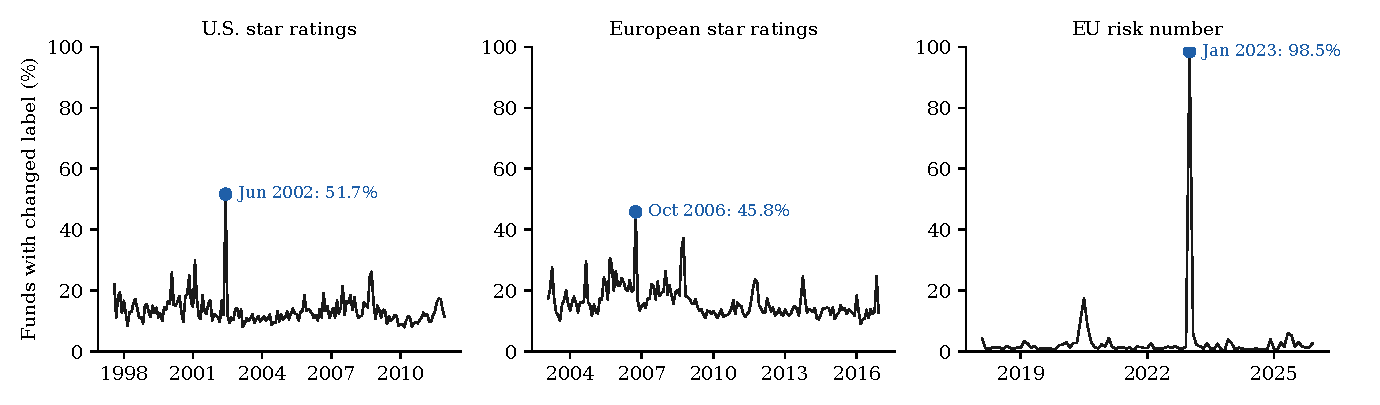
\includegraphics[width=\textwidth]{figurer/figur1.pdf}
\caption{Share of funds whose label differs from the month before. Left: Morningstar ratings of U.S. funds; Morningstar began rating within category peer groups on 30 June 2002. Middle: Morningstar ratings of European funds; on 31 October 2006 Morningstar introduced five- and ten-year ratings in Europe and made the overall rating a weighted average of the three-, five- and ten-year ratings. Right: the EU risk number; the Summary Risk Indicator replaced the Synthetic Risk and Reward Indicator on 1 January 2023.}
\end{figure}

\begin{table}[H]
\caption{Two rating reforms in the form of Table 4 of Ben-David et al.\ (2022). The first row of each panel gives the share of fund-months in which the fund's rating differs from its previous observation in the sample. ``Explained by month $\times$ rating'' is the $R^2$ of a regression of flow on the 18-month raw return with month-by-rating effects, minus the $R^2$ with month effects only; ``category beyond rating'' adds month-by-category effects to month-by-rating effects. The event month counts as before. Panel A: Morningstar began rating U.S. funds within category peer groups on 30 June 2002. Panel B: on 31 October 2006 Morningstar introduced five- and ten-year ratings in Europe and made the overall rating a weighted average of the three-, five- and ten-year ratings (Morningstar 2023, Appendix 2).}
\centering\resizebox{\textwidth}{!}{\begin{tabular}{lccc}
\toprule
 & Before & Event month & After \\
\midrule
\multicolumn{4}{l}{\textit{Panel A. United States, June 2002}} \\
Funds with changed rating, percent per month: Ben-David et al. & 13.9 & 54.2 & 11.9 \\
Funds with changed rating, percent per month: ours & 14.0 & 53.0 & 12.1 \\
Explained by month $\times$ rating: Ben-David et al. & 0.073 & & 0.074 \\
Explained by month $\times$ rating: ours & 0.064 & & 0.060 \\
Explained by month $\times$ category: Ben-David et al. & 0.043 & & 0.015 \\
Explained by month $\times$ category: ours & 0.037 & & 0.017 \\
Category beyond rating: Ben-David et al. & 0.022 & & 0.014 \\
Category beyond rating: ours & 0.023 & & 0.013 \\
\addlinespace
\multicolumn{4}{l}{\textit{Panel B. Europe, October 2006}} \\
Funds with changed rating, percent per month & 20.3 & 48.0 & 14.6 \\
Explained by month $\times$ rating & 0.0138 & & 0.0097 \\
Fund-months & 24,924 & 1,130 funds & 192,690 \\
\bottomrule
\end{tabular}
}
\end{table}
\raknas Andel med ändrat betyg: andelen fondmånader där betyget skiljer sig från fondens föregående rad i urvalet, räknad över alla fondmånader före respektive efter (kodens \kod{lag1(rating)} och \kod{proc summary ... by ba\_reform}). Förklaringsgrad (vanligt $R^2$ i de två regressionerna; observationer som är ensamma i sin grupp tas bort, som Statas \kod{reghdfe} gör):
\begin{equation}
R^2_{\text{marg}}=R^2\big(F\ \text{på}\ \text{ALPHA}^{\text{rå}},\ \mu_{t\times\text{betyg}}\big)-R^2\big(F\ \text{på}\ \text{ALPHA}^{\text{rå}},\ \mu_t\big).
\end{equation}
\kalla{[BD] tabell 4, s.~1746, och texten s.~1746--1748; [BD-kod] ``Table 4. Effects of Morningstar's Reform on Ratings and Flows'': \kod{af\_j02 = 1; if yyyymm le 200206 then af\_j02 = 0}, \kod{reghdfe std\_floww retrf\_a if af\_j02 == 0, a(yyyymm)} mot \kod{a(month\_rating)}. Kategoriraderna tas bara med för USA: de prövar innehållet i 2002 års reform. Kod: \kod{lib/ankartest.py:andel\_andrad, table4b}; \kod{test/usa.py}, \kod{test/eu2006.py}.}
\visar I USA är betygets förklaringsgrad oförändrad efter reformen, som hos ankaret. I Europa bytte 48,0~\% av fonderna betyg i oktober 2006, mot 20,3~\% en vanlig månad före. Betygets förklaringsgrad är 0,0138 före och 0,0097 efter. Talen är små: en del av dem uppstår av sig själv när grupperna blir fler, så skillnaden ska inte läsas som ett säkert fall.
\kalla{Händelserna: [MS] bilaga 2, s.~19. 31 oktober 2006, Europa: fem- och tioårsbetyg infördes, totalbetyget blev ett vägt medel av tre-, fem- och tioårsbetygen, och uppskjutna avgifter och inlösenavgifter började räknas in. \textbf{Två saker ändrades alltså samma dag.} Fonder med under fem års historik behåller treårsbetyget som totalbetyg ([MS] exhibit 5, s.~15). 30 juni 2002, USA: jämförelse inom kategori, och tre ändringar till. Morningstar ändrade metoden igen 31 oktober 2016 (avgiftsjusteringen togs bort); Europapanelen slutar där.}

\setcounter{figure}{2}
\begin{figure}[H]
\centering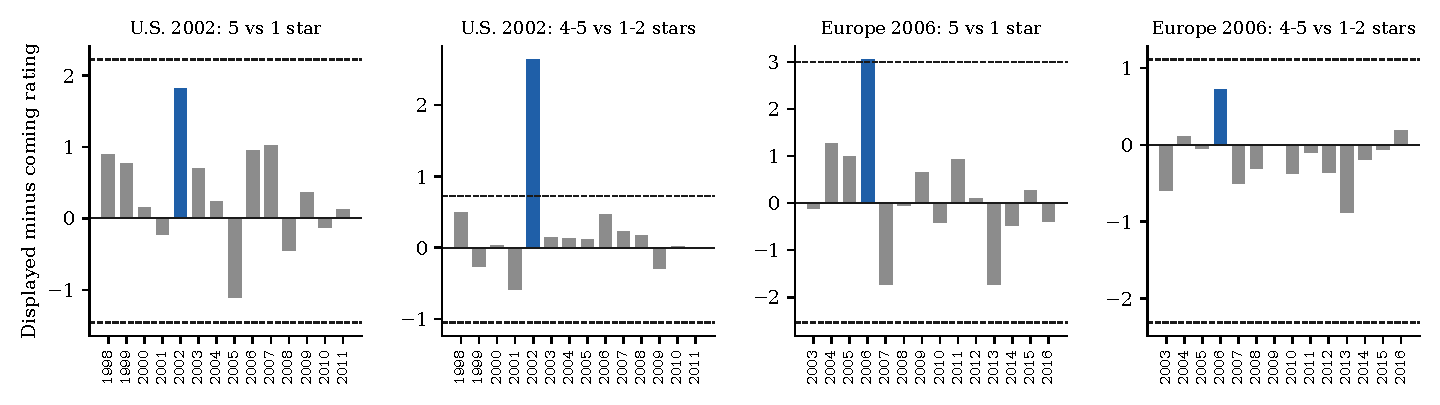
\includegraphics[width=\textwidth]{figurer/figur3.pdf}
\caption{Did flows follow the displayed rating or the coming one? The statistic is equation 2 of Ben-David et al.\ (2022): the flow spread between top-rated and bottom-rated funds, sorted on the displayed rating, minus the same spread sorted on the rating the fund has in the reform month, summed over the three months before the reform month. The blue bar is the reform year; grey bars are other years, treated as placebos. Dashed lines are the 1st and 99th percentiles of a bootstrap over the placebo years. United States: March to May, June rating. Europe: July to September, October rating. The layout follows their Figure 5, Panel B.}
\end{figure}
\raknas För månad $m$ i de tre månaderna före händelsemånaden, år $y$:
\begin{equation}
D_y=\sum_{m}\Big[\big(\bar F^{\,\text{visat}}_{\text{topp},m}-\bar F^{\,\text{visat}}_{\text{botten},m}\big)-\big(\bar F^{\,\text{kommande}}_{\text{topp},m}-\bar F^{\,\text{kommande}}_{\text{botten},m}\big)\Big].
\end{equation}
Intervallet: dra ett jämförelseår, dra tre av dess månader med återläggning, summera; 10~000 dragningar; 1:a och 99:e percentilen. Antalet dragningar anger ankaret inte. Fonden ska finnas i urvalet i händelsemånaden, och dess betyg den månaden är det kommande betyget (kodens \kod{focal\_rating}). Alla andra år är jämförelseår.
\kalla{[BD] ekvation 2, s.~1749; figur 5, panel B, s.~1747 (``Years other than 2002 serve as placebo tests''); bootstrap enligt not 24, s.~1749 (``we first resample the focal year and then randomly draw 3 months within that year (with replacement)''); [BD-kod] ``Test For Figure 5 Panel B''. Kod: \kod{lib/ankartest.py:fig5b}.}
\begin{center}\resizebox{0.95\textwidth}{!}{\begin{tabular}{lccccc}
\toprule
 & Event year & 1st percentile & 99th percentile & Position & Rank among years \\
\midrule
United States 2002, 5 against 1 star & 1.82 & $-$1.46 & 2.22 & inside & 1 of 14 \\
United States 2002, 4--5 against 1--2 stars & 2.64 & $-$1.05 & 0.72 & above & 1 of 14 \\
Europe 2006, 5 against 1 star & 3.05 & $-$2.54 & 2.99 & above & 1 of 14 \\
Europe 2006, 4--5 against 1--2 stars & 0.72 & $-$2.31 & 1.11 & inside & 1 of 14 \\
\bottomrule
\end{tabular}
}\end{center}
\visar I USA 2002 följde flödena det visade betyget, inte det kommande: måttet för 4--5 mot 1--2 stjärnor ligger över intervallet och är störst av alla år. \textbf{Ankaret ligger över gränsen i båda rutorna; vi i en.} Ankarets staplar är 2,84 (5 mot 1) och 1,81 (4--5 mot 1--2), summerade ur kodens utskrift, mot övre gränser på ungefär 1,3 och 0,4, avlästa ur deras figur 5 B. Vår stapel för 5 mot 1 är 2,47, nära ankarets, men vår gräns är högre (3,11), eftersom våra jämförelseår svänger mer. I Europa 2006 är båda måtten störst av alla år och båda ligger över intervallet (4,91 mot gränsen 4,08, och 0,89 mot 0,52). Gränserna är vida, eftersom perioden före bytet är kort.

\section{Följer flödena risksiffran?}
\begin{table}[H]
\caption{The risk number as a third signal. Monthly flow (percent of assets) is regressed on the displayed risk number (1 to 7), the star rating (1 to 5), the 18-month raw return, flow 19 months earlier, log size, log age, expense ratio and 60-month return volatility. Coefficients are multiplied by 12. Fama-MacBeth rows average monthly cross-sectional coefficients, with Newey-West standard errors (six lags); the pooled row has month effects and standard errors clustered by fund and month. Panel B gives the $R^2$ with all three blocks minus the $R^2$ without the block named, with month effects and indicator variables for ratings and risk numbers. European equity funds, June 2019 to December 2025.}
\centering\begin{tabular}{lcccccc}
\toprule
 & \multicolumn{3}{c}{Risk number} & \multicolumn{2}{c}{Star rating} & Fund-months \\
 & Coef. & s.e. & 95\% interval & Coef. & $t$ & \\
\midrule
\multicolumn{7}{l}{\textit{Panel A. Percentage points of assets per year, per risk class or per star}} \\
Fama-MacBeth & 0.61 & 0.66 & [$-$0.67, 1.90] & 5.53 & 11.9 & 66,365 \\
Pooled, month effects & 0.80 & 0.98 & [$-$1.11, 2.72] & 5.68 & 10.7 & 66,365 \\
\addlinespace
\multicolumn{7}{l}{\textit{Panel B. Share of flow variation explained beyond the other two blocks (percent, equal-weighted)}} \\
\multicolumn{7}{l}{Past return 1.20 \quad Star rating 0.67 \quad Risk number 0.02 \quad (118,102 fund-months)} \\
\bottomrule
\end{tabular}

\end{table}
\raknas Varje månad $t$: $F_{p,t}=a_t+b_t\,\text{Risk}_{p,t}+c_t\,\text{Betyg}_{p,t}+\gamma_t'X_{p,t}+e_{p,t}$. Skattningen är $\bar b=\frac1T\sum_t b_t$ med Newey-West-fel.
\kalla{Regressionen är [BD] figur 5 A(b) med risksiffran tillagd (se ovan). Fama-MacBeth när signaler jämförs: [BD] bilaga B.3, s.~1767, och tabell 6, kolumn 4, s.~1761; [BD-kod] ``Table 6, Column 4: Run Return Decomposition Regression usign Fama-MachBeth''; [FM]. Kod: \kod{test/eu.py:tredje\_signal}, \kod{lib/stat.py:fama\_macbeth}.}
\visar Risksiffran har inget säkert samband med flödena utöver stjärnan och avkastningen: $+1{,}08$ med intervallet $-0{,}22$ till $+2{,}37$. Även vid intervallets övre gräns är ett risksteg värt mindre än hälften av en stjärna (5,10). Det är ett samband, inte en orsak. Regressionen bygger på drygt hälften av fondmånaderna, eftersom någon kontrollvariabel saknas för resten.

\begin{table}[H]
\caption{The January 2023 switch in the form of Table 4 of Ben-David et al.\ (2022). The first row gives the share of funds whose displayed risk number differs from the month before. The next rows give the $R^2$ of a regression of flow on the 18-month raw return with month-by-label effects, minus the $R^2$ with month effects only; ``beyond'' adds month-by-risk-number effects to month-by-rating effects. Before is June 2019 to December 2022, after is January 2023 to December 2025.}
\centering\begin{tabular}{lccc}
\toprule
 & Before & January 2023 & After \\
\midrule
Funds with changed risk number, percent per month & 2.2 & 98.5 & 1.9 \\
Explained by month $\times$ risk number & 0.0040 & & 0.0044 \\
Explained by month $\times$ star rating & 0.0109 & & 0.0130 \\
Risk number beyond star rating & 0.0040 & & 0.0040 \\
Fund-months & 48,142 & 923 funds & 36,243 \\
\bottomrule
\end{tabular}

\end{table}
\kalla{Samma formler och källor som tabell 3, panel A och B, med risksiffran som etikett. Kod: \kod{test/eu.py:handelse2023}.}

\begin{table}[H]
\caption{Did funds whose risk number fell further receive more flow? Fund-month regressions of monthly flow (percent of assets) on Fall $\times$ After, where Fall is the number of classes the fund's risk number fell on 1 January 2023 (0, 1 or 2) and After is one from January 2023. Coefficients are multiplied by 12 and read as percentage points of assets per year. The specification follows equation 1 of Adelino, Cunha, and Ferreira (2017): column 1 has fund and category-by-month effects, column 2 adds volatility-decile-by-month effects, and column 3 adds the star rating as a control. Standard errors, in parentheses, are clustered by fund. The minimum detectable effect is 2.8 standard errors. January 2021 to December 2024. Flows are summed over the fund's non-institutional share classes that are not sold only in the United Kingdom, and winsorized at the 1st and 99th percentiles within month.}
\centering\begin{tabular}{lccc}
\toprule
 & (1) & (2) & (3) \\
 & & Main & With star rating \\
\midrule
Fall $\times$ After & 0.64 & 0.01 & $-$0.55 \\
 & (0.79) & (0.82) & (0.86) \\
Star rating & & & 5.99 \\
 & & & (0.33) \\
\addlinespace
95\% interval & [$-$0.90, 2.18] & [$-$1.60, 1.62] & [$-$2.22, 1.13] \\
Minimum detectable effect & 2.2 & 2.3 & 2.4 \\
\addlinespace
Fund effects & Yes & Yes & Yes \\
Category $\times$ month effects & Yes & Yes & Yes \\
Volatility decile $\times$ month effects & No & Yes & Yes \\
Funds & 4,818 & 4,818 & 4,277 \\
Fund-months & 230,531 & 230,531 & 197,296 \\
\bottomrule
\end{tabular}

\end{table}
\raknas
\begin{equation}
F_{f,t}=\beta\,\text{Fall}_f\times\text{After}_t+\eta_f+\eta_{\text{kategori},t}+\eta_{\text{volatilitetsdecil},t}+\varepsilon_{f,t}.
\end{equation}
$\text{Fall}_f$ = gammal siffra (SRRI, december 2022) minus ny (SRI). Volatilitetsdecilen bygger på fondens volatilitet före bytet. Minsta påvisbara effekt: $(1{,}96+0{,}84)\cdot SE=2{,}8\cdot SE$ (5~\% nivå, 80~\% styrka).
\kalla{[ACF] ekvation 1, s.~3236: $\text{Rating}_{it}=\beta\,\text{Recalibrated}_i\times\text{Post}_t+\text{kontroller}+\eta_i+\eta_{\text{state},t}+\eta_{\text{size},t}+\varepsilon_{it}$, med standardfel klustrade på county och storleksdecilen med ``in some specifications''. Deras förklarande variabel är andelen uppgraderade kommuner i countyt (ekvation 1) eller en dummy för uppgraderad kommun (ekvation 2, s.~3237). \textbf{Vi räknar i stället antal steg siffran föll (0, 1, 2)}, eftersom bara 418 av 4~818 fonder föll inget steg. Vår översättning i övrigt: fond för county, kategori $\times$ månad för delstat $\times$ år, volatilitetsdecil $\times$ månad för storleksdecil $\times$ år. Deras skäl för storleksdecilen är att fånga tidsvarierande faktorer som träffar olika stora enheter olika (s.~3236). Hos oss bestämmer volatiliteten hur många steg siffran föll, därför får den egna tidseffekter. Winsoriseringen är ankarets ([BD] s.~1733). Minsta påvisbara effekt krävs av kursens bilder; \textbf{formeln saknar källa i underlaget}. Kod: \kod{test/byte2023.py}.}
\visar Ingen effekt hittas. Intervallet i kolumn 2 utesluter effekter större än ungefär en fjärdedel av det en stjärna hänger ihop med i kolumn 3.

\setcounter{figure}{3}
\begin{figure}[H]
\centering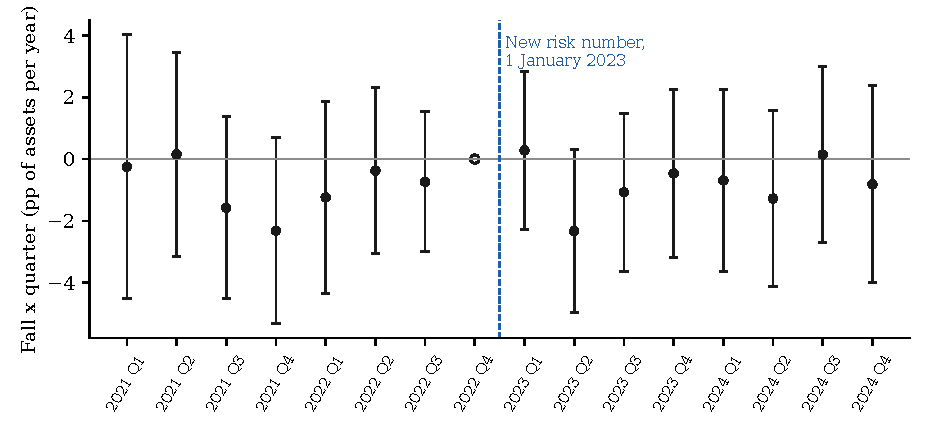
\includegraphics[width=0.72\textwidth]{figurer/figur4.pdf}
\caption{Fall $\times$ quarter. Coefficients from the regression in Table 6, column 2, with Fall interacted with an indicator for each quarter; the fourth quarter of 2022 is the base. Bars are 95 percent intervals, standard errors clustered by fund.}
\end{figure}
\kalla{[ACF] figur 4, s.~3243 (koefficienter per händelseår; ``no evidence of significant preexisting differential trends'', s.~3242). Kod: \kod{test/byte2023.py}, avsnittet ``handelsestudie''.}
\begin{center}\resizebox{0.95\textwidth}{!}{\begin{tabular}{lcccccccc}
\toprule
Quarter & 2021 Q1 & 2021 Q2 & 2021 Q3 & 2021 Q4 & 2022 Q1 & 2022 Q2 & 2022 Q3 &  \\
Coef. & $-$0.25 & 0.15 & $-$1.58 & $-$2.32 & $-$1.24 & $-$0.38 & $-$0.74 &  \\
s.e. & (2.18) & (1.68) & (1.50) & (1.54) & (1.58) & (1.37) & (1.16) &  \\
\addlinespace
Quarter & 2023 Q1 & 2023 Q2 & 2023 Q3 & 2023 Q4 & 2024 Q1 & 2024 Q2 & 2024 Q3 & 2024 Q4 \\
Coef. & 0.28 & $-$2.33 & $-$1.08 & $-$0.46 & $-$0.69 & $-$1.28 & 0.14 & $-$0.81 \\
s.e. & (1.30) & (1.34) & (1.31) & (1.39) & (1.50) & (1.45) & (1.45) & (1.63) \\
\addlinespace
\multicolumn{9}{l}{Wald test that all coefficients are zero: before the switch $p$ = 0.71; after $p$ = 0.49} \\
\bottomrule
\end{tabular}
}\end{center}

\clearpage
\section{Bilaga}
\begin{table}[H]
\caption*{\textbf{Table A1.} All ten pairs of Table 3 in Ben-David et al.\ (2022). See Table 2 for definitions. The three blocks use the monthly flow in percent of assets, the monthly flow in USD million, and an indicator for a positive flow (coefficients in percentage points).}
\centering\footnotesize\begin{tabular}{lcccccc}
\toprule
 & \multicolumn{2}{c}{Ben-David et al.} & \multicolumn{2}{c}{United States, ours} & \multicolumn{2}{c}{Europe, ours} \\
 & Coef. & $t$ & Coef. & $t$ & Coef. & $t$ \\
\midrule
\multicolumn{7}{l}{\textit{Flow, percent of assets per month}} \\
Star rating vs Raw & 0.099 & (2.50) & 0.280 & (4.46) & $-$0.076 & ($-$0.97) \\
Star rating vs CAPM & 0.108 & (2.72) & 0.262 & (4.29) & $-$0.091 & ($-$1.18) \\
Star rating vs FF3 & 0.192 & (4.85) & 0.412 & (6.68) & 0.121 & (1.76) \\
Star rating vs FFC & 0.188 & (4.73) & 0.346 & (5.81) & 0.120 & (1.68) \\
Raw vs CAPM & 0.032 & (0.62) & $-$0.054 & ($-$0.66) & $-$0.066 & ($-$0.52) \\
Raw vs FF3 & 0.207 & (4.74) & 0.211 & (2.97) & 0.416 & (4.40) \\
Raw vs FFC & 0.195 & (4.48) & 0.097 & (1.47) & 0.407 & (4.19) \\
CAPM vs FF3 & 0.220 & (5.06) & 0.257 & (3.53) & 0.521 & (5.59) \\
CAPM vs FFC & 0.197 & (4.55) & 0.129 & (2.03) & 0.500 & (5.18) \\
FF3 vs FFC & $-$0.017 & ($-$0.26) & $-$0.251 & ($-$3.08) & $-$0.008 & ($-$0.06) \\
\addlinespace
\multicolumn{7}{l}{\textit{Flow, USD million per month}} \\
Star rating vs Raw & 10.9 & (6.27) & 7.7 & (7.11) & $-$0.1 & ($-$0.62) \\
Star rating vs CAPM & 11.0 & (6.26) & 7.5 & (6.84) & $-$0.2 & ($-$0.98) \\
Star rating vs FF3 & 12.3 & (7.19) & 9.3 & (8.10) & 0.4 & (1.65) \\
Star rating vs FFC & 12.5 & (7.09) & 9.0 & (7.96) & 0.4 & (1.50) \\
Raw vs CAPM & 0.3 & (0.37) & $-$0.4 & ($-$0.49) & $-$0.4 & ($-$1.32) \\
Raw vs FF3 & 3.1 & (2.84) & 2.5 & (2.95) & 1.2 & (3.82) \\
Raw vs FFC & 3.7 & (2.69) & 1.9 & (2.27) & 1.1 & (3.57) \\
CAPM vs FF3 & 3.4 & (2.99) & 2.9 & (3.21) & 1.6 & (4.97) \\
CAPM vs FFC & 3.9 & (2.79) & 2.2 & (2.51) & 1.4 & (4.57) \\
FF3 vs FFC & 1.7 & (0.85) & $-$1.1 & ($-$1.12) & $-$0.3 & ($-$0.72) \\
\addlinespace
\multicolumn{7}{l}{\textit{Probability of a positive flow, percentage points}} \\
Star rating vs Raw & 7.1 & (4.45) & 5.2 & (7.33) & 0.1 & (0.08) \\
Star rating vs CAPM & 7.3 & (4.57) & 5.0 & (6.95) & $-$0.1 & ($-$0.10) \\
Star rating vs FF3 & 10.4 & (6.55) & 7.2 & (10.04) & 2.5 & (3.18) \\
Star rating vs FFC & 10.0 & (6.26) & 6.6 & (9.42) & 2.4 & (3.06) \\
Raw vs CAPM & 0.8 & (0.41) & $-$0.8 & ($-$0.78) & $-$0.6 & ($-$0.63) \\
Raw vs FF3 & 7.3 & (4.41) & 3.1 & (3.80) & 5.1 & (5.12) \\
Raw vs FFC & 6.5 & (3.97) & 2.0 & (2.62) & 4.8 & (4.92) \\
CAPM vs FF3 & 8.0 & (4.71) & 3.7 & (4.27) & 6.3 & (6.24) \\
CAPM vs FFC & 6.8 & (4.07) & 2.5 & (3.10) & 5.9 & (5.97) \\
FF3 vs FFC & $-$1.4 & ($-$0.56) & $-$2.3 & ($-$2.47) & $-$0.7 & ($-$0.65) \\
\addlinespace
\bottomrule
\end{tabular}

\end{table}

\begin{table}[H]
\caption*{\textbf{Table A2.} Aggregate flows (Table 2, columns 1 to 5, of Ben-David et al.\ 2022). Time-series regressions of the equal-weighted average monthly flow (percent) on the equal-weighted average raw return and, in columns 2 to 5, one further return measure. Regressors are standardized. Newey-West $t$-statistics with six lags.}
\centering\begin{tabular}{llcccccc}
\toprule
 & & \multicolumn{2}{c}{Ben-David et al.} & \multicolumn{2}{c}{United States, ours} & \multicolumn{2}{c}{Europe, ours} \\
Column & Regressor & Coef. & $t$ & Coef. & $t$ & Coef. & $t$ \\
\midrule
(1) & Raw return & 0.179 & (4.47) & 0.130 & (2.41) & 0.234 & (2.26) \\
(2) & Raw return & 0.176 & (4.05) & 0.125 & (2.39) & 0.234 & (2.31) \\
 & Market-adjusted & 0.015 & (0.26) & 0.092 & (1.39) & 0.000 & (0.01) \\
(3) & Raw return & 0.178 & (4.35) & 0.137 & (2.60) & 0.245 & (2.33) \\
 & CAPM & 0.018 & (0.38) & 0.087 & (1.47) & $-$0.028 & ($-$0.53) \\
(4) & Raw return & 0.186 & (4.60) & 0.130 & (2.41) & 0.272 & (2.52) \\
 & FF3 & $-$0.048 & ($-$1.01) & $-$0.017 & ($-$0.26) & $-$0.104 & ($-$1.77) \\
(5) & Raw return & 0.182 & (4.44) & 0.130 & (2.40) & 0.288 & (2.54) \\
 & FFC & $-$0.018 & ($-$0.36) & 0.029 & (0.49) & $-$0.130 & ($-$1.87) \\
Months & & \multicolumn{2}{c}{175} & \multicolumn{2}{c}{174} & \multicolumn{2}{c}{79} \\
\bottomrule
\end{tabular}

\end{table}
\kalla{[BD] tabell 2, s.~1737; [BD-kod] ``Code and Output for Table 2'' (\kod{newey pflow\_mmew100 retrf\_mmew\_z retexmkt\_mmew\_z, lag(6)} och så vidare). Standardfelen har faktorn $n/(n-k)$ som Statas \kod{newey}; Statas manual är inte läst i denna körning. Kod: \kod{lib/ankartest.py:table2}, \kod{lib/stat.py:nw\_reg}.}

\begin{table}[H]
\caption*{\textbf{Table A3.} Flows to top-ranked funds (Figure 4 of Ben-David et al.\ 2022). Average monthly flow and share of funds with a positive flow among the funds ranked at the top by each measure.}
\centering\begin{tabular}{lcccccc}
\toprule
 & \multicolumn{2}{c}{Ben-David et al.} & \multicolumn{2}{c}{United States, ours} & \multicolumn{2}{c}{Europe, ours} \\
Top funds by & Flow (\%) & Positive (\%) & Flow (\%) & Positive (\%) & Flow (\%) & Positive (\%) \\
\midrule
Star rating & 1.16 & 67.5 & 2.47 & 71.6 & 0.83 & 53.7 \\
Raw & 0.99 & 61.7 & 2.06 & 64.1 & 0.92 & 53.4 \\
CAPM & 0.98 & 61.5 & 2.09 & 64.5 & 0.93 & 53.6 \\
FF3 & 0.84 & 58.9 & 1.86 & 61.2 & 0.60 & 49.5 \\
FFC & 0.84 & 59.0 & 1.95 & 62.0 & 0.61 & 49.6 \\
All funds & $-$0.49 & 35.2 & $-$0.15 & 39.0 & $-$0.48 & 38.9 \\
\bottomrule
\end{tabular}

\end{table}
\kalla{[BD] figur 4, s.~1743. Ankarets tal är hämtade ur kodens utskrift (\kod{fig4\_panela}, \kod{average\_all}). Kod: \kod{lib/ankartest.py:fig4}.}

\begin{table}[H]
\caption*{\textbf{Table A4.} Table 2, Panel A, on other data: all share classes with an EU fact sheet (not only those sold in the EEA outside the United Kingdom), and Fama-French European factors instead of Developed factors.}
\centering\begin{tabular}{lcccc}
\toprule
 & \multicolumn{2}{c}{Europe, all KID classes} & \multicolumn{2}{c}{Europe, European factors} \\
 & Coef. & $t$ & Coef. & $t$ \\
\midrule
Star rating vs Raw & $-$0.012 & ($-$0.19) &  &  \\
Star rating vs CAPM & $-$0.025 & ($-$0.41) & $-$0.137 & ($-$1.50) \\
Star rating vs FF3 & 0.170 & (3.08) & 0.011 & (0.13) \\
Star rating vs FFC & 0.165 & (2.89) & 0.002 & (0.03) \\
Fund-months & \multicolumn{2}{c}{182,975} & \multicolumn{2}{c}{94,203} \\
\bottomrule
\end{tabular}

\end{table}

\begin{table}[H]
\caption*{\textbf{Table A4, continued.} Table 3 of Ben-David et al.\ (2022) in four forms. ``Code form'' regresses flow on Top$^A-$Top$^B$ and an indicator for being top-ranked by either measure, without month effects. The next two columns replace the second regressor with an indicator for being top-ranked by both, and with the sum of the two indicators. ``Text form'' regresses flow on the two indicators with month effects and reports the difference between their coefficients, as the printed table note describes. $t$-statistics use standard errors clustered by fund and month.}
\centering\resizebox{\textwidth}{!}{\begin{tabular}{lcccccccc}
\toprule
 & \multicolumn{2}{c}{Code form (main)} & \multicolumn{2}{c}{Second regressor: both} & \multicolumn{2}{c}{Second regressor: sum} & \multicolumn{2}{c}{Text form} \\
 & $b_1$ & $t$ & $b_1$ & $t$ & $b_1$ & $t$ & $c_A-c_B$ & $t$ \\
\midrule
\multicolumn{9}{l}{\textit{United States}} \\
Star rating vs Raw & 0.217 & (3.26) & 0.217 & (2.65) & 0.217 & (3.30) & 0.434 & (3.33) \\
Star rating vs CAPM & 0.181 & (2.80) & 0.181 & (2.23) & 0.181 & (2.83) & 0.363 & (2.85) \\
Star rating vs FF3 & 0.327 & (5.09) & 0.327 & (4.34) & 0.327 & (5.17) & 0.654 & (5.22) \\
Star rating vs FFC & 0.303 & (4.85) & 0.303 & (4.08) & 0.303 & (4.93) & 0.607 & (4.96) \\
Raw vs CAPM & $-$0.107 & ($-$1.17) & $-$0.107 & ($-$1.09) & $-$0.107 & ($-$1.16) & $-$0.214 & ($-$1.16) \\
Raw vs FF3 & 0.185 & (2.65) & 0.185 & (2.44) & 0.185 & (2.65) & 0.370 & (2.67) \\
\addlinespace
\multicolumn{9}{l}{\textit{Europe}} \\
Star rating vs Raw & $-$0.081 & ($-$0.88) & $-$0.081 & ($-$0.83) & $-$0.081 & ($-$0.88) & $-$0.162 & ($-$0.88) \\
Star rating vs CAPM & $-$0.100 & ($-$1.12) & $-$0.100 & ($-$1.06) & $-$0.100 & ($-$1.12) & $-$0.201 & ($-$1.13) \\
Star rating vs FF3 & 0.042 & (0.52) & 0.042 & (0.48) & 0.042 & (0.52) & 0.083 & (0.52) \\
Star rating vs FFC & 0.075 & (0.91) & 0.075 & (0.85) & 0.075 & (0.91) & 0.151 & (0.92) \\
Raw vs CAPM & $-$0.085 & ($-$0.56) & $-$0.085 & ($-$0.54) & $-$0.085 & ($-$0.56) & $-$0.169 & ($-$0.56) \\
Raw vs FF3 & 0.258 & (2.33) & 0.258 & (2.27) & 0.258 & (2.33) & 0.515 & (2.34) \\
\addlinespace
\bottomrule
\end{tabular}
}
\end{table}
\kalla{[BD] tabell 3, not, s.~1744 (``the difference in the coefficients of the first and the second indicators'', ``controlling for month fixed effects''); [BD-kod] ``Table 3 (Flows to Top-Ranked Funds: Horse Races Between Performance Measures)''. Kod: \kod{test/tabell3\_former.py}.}
\visar $b_1$ är densamma hur den andra regressorn än definieras. Textens form ger exakt det dubbla med i stort sett samma $t$-värde. Valet av form ändrar alltså ingen slutsats; det ändrar bara skalan med en faktor två.

\begin{table}[H]
\caption*{\textbf{Table A5.} Table 6, column 2, with Fall replaced by indicators for a fall of one class and of two classes. Adelino et al.\ (2017) report the same split by notch (Internet Appendix Table IA.5, referred to on p.~3242).}
\centering\begin{tabular}{lccccc}
\toprule
 & Coef. & s.e. & 95\% interval & Funds & Fund-months \\
\midrule
One class $\times$ After & 2.47 & 2.06 & [$-$1.56, 6.50] & 4,818 & 230,531 \\
Two classes $\times$ After & 1.70 & 2.16 & [$-$2.53, 5.92] & 4,818 & 230,531 \\
\bottomrule
\end{tabular}

\end{table}

\begin{table}[H]
\caption*{\textbf{Table A6.} Europe, October 2006: three ways of combining the two data sources for assets. See Table 3 and Figure 3 for definitions.}
\centering\resizebox{\textwidth}{!}{\begin{tabular}{lccc}
\toprule
 & Morningstar first, LSEG fills & LSEG first & Morningstar only \\
\midrule
Fund-months & 296,337 & 296,525 & 254,710 \\
Fund-months before the change & 57,043 & 57,123 & 24,432 \\
\addlinespace
Funds with changed rating: before / October 2006 / after & 19.0 / 45.8 / 15.3 & 19.0 / 45.5 / 15.3 & 20.7 / 45.3 / 15.1 \\
Explained by month $\times$ rating: before / after & 0.0119 / 0.0100 & 0.0122 / 0.0098 & 0.0161 / 0.0102 \\
\addlinespace
\multicolumn{4}{l}{\textit{Displayed minus coming rating, 2006, with bootstrap interval and rank among years}} \\
5 against 1 star & 3.05 [$-$2.54, 2.99], 1/14 & 3.50 [$-$2.51, 2.52], 1/14 & 1.82 [$-$4.44, 1.47], 1/14 \\
4--5 against 1--2 stars & 0.72 [$-$2.31, 1.11], 1/14 & 0.67 [$-$1.82, 1.06], 1/14 & 0.33 [$-$6.92, 6.68], 2/14 \\
\bottomrule
\end{tabular}
}
\end{table}

\visar Ordningen mellan källorna spelar liten roll. Utan LSEG:s förmögenhet finns 12~988 fondmånader före bytet i stället för 24~924.

\begin{figure}[H]
\centering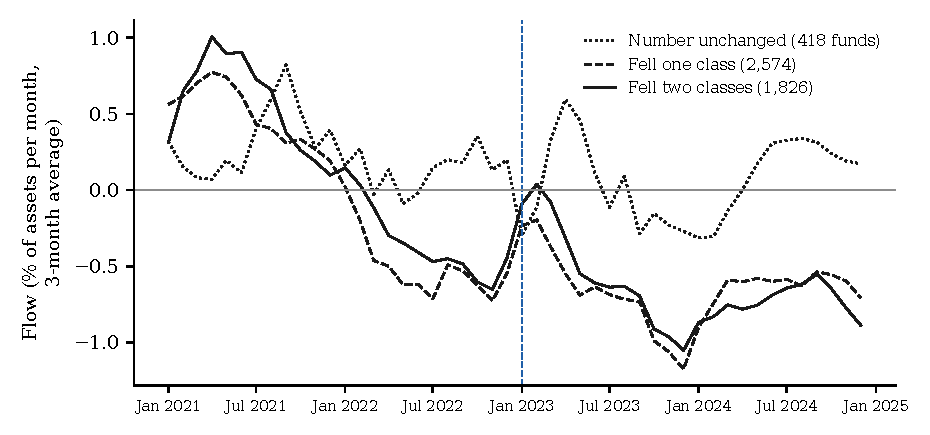
\includegraphics[width=0.72\textwidth]{figurer/figur_a1.pdf}
\caption*{\textbf{Figure A7.} Average monthly flow by how far the risk number fell, three-month moving average. The dashed line marks 1 January 2023.}
\end{figure}

\textbf{UK mot EU.} Inte återskapad i \kod{final\_code}. Talen från körningen 19 november står i \kod{RESULTAT\_omkorning\_full2\_ny\_B2\_2026-11-19}, avsnitt 5 (huvudnivå: $+1{,}17$, SE $1{,}33$, 459 fonder). Skripten ligger i \kod{analys\_eu\_full2\_2026-11-19/}.

\section{Avvikelser från ankaret}\label{sec:avvik}
\begin{tabular}{@{}p{0.5cm}p{6.9cm}p{7.9cm}@{}}
\toprule
 & Ankaret & Vi \\
\midrule
1 & Urvalet är Barber, Huang och Odeans fondmånader ur CRSP ([BD-kod], kodens huvud), sammanslaget med Morningstar ([BD] s.~1733) & Eget urval ur Morningstar Direct, byggt efter deras regler. Flödena sprider 1,6 gånger mer (tabell 1, panel A). Se avsnittet om urvalen \\
2 & Tabell 3 enligt texten: skillnad mellan två indikatorers koefficienter ([BD] s.~1744) & Kodens form: $b_1$ på skillnaden mellan indikatorerna, utan månadseffekt. Det är halva skillnaden och det tal ankaret trycker. Textens form står i bilaga A4 \\
3 & Betor på 60 månader ([BD] ekvation A.2, s.~1765); fem års avkastningshistorik krävs ([BHO] not 8); minst 36 observationer i fönstret ([BD-kod]) & Samma tre regler i alla urval sedan 21 november. Följd: Europa börjar juni 2019, eftersom avkastningen i exporten börjar 2013, och Europa 2006 börjar juni 2004 \\
4 & Historisk avgift och kategori & Dagens avgift och kategori (det exporten ger) \\
5 & Amerikanska faktorer & Europa: Fama-Frenchs Developed-faktorer i USD (Europe-faktorer i bilaga A4) \\
6 & Diversifierade amerikanska aktiefonder & Europa: alla aktiefonder med säte i Luxemburg eller Irland \\
7 & Kontroller i figur 5 A(b): se figur 2 & Europa 2004--2016 har bara rå avkastning som kontroll (panelen saknar de övriga) \\
8 & Fonder med minst 10 MUSD, alla andelsklasser & Tabell 6: icke-institutionella klasser med minst 1 MUSD och minst 18 flödesmånader på var sida om bytet. \textbf{Eget urvalsval; se sista avsnittet} \\
9 & Kodens utskrifter har 175 månader (från juni 1997); texten anger juli 1997 ([BD] s.~1734) & Juli 1997 till december 2011, 174 månader \\
10 & Avsnitt 4 (tabell 5 och 6, figur 6--8) & Replikeras inte \\
\bottomrule
\end{tabular}

\section{Kontroll av att talen stämmer}
\begin{itemize}[leftmargin=*,itemsep=1pt]
\item Hela kedjan är körd från rådata i en ren kopia med repots mappstruktur. Alla paneler utom den för tabell 6 byggdes om från rådata 21 november med femårskravet. Testen kördes sedan två gånger och gav identiska filer (83 i \kod{final\_result/tal/}, 16 tabellfiler).
\item Varje funktion i \kod{lib/ankartest.py} är läst mot motsvarande avsnitt i författarnas kod. Skillnaderna som hittades står på första sidan och i \kod{final\_code/KONTROLL.md}.
\item Ankarets egna tal är inskrivna för hand och kontrollerade mot den tryckta artikeln (tabell 1, s.~1734; tabell 3, s.~1744; tabell 4, s.~1746) och mot utskrifterna i författarnas kod (tabell 2, figur 3, figur 4). \textbf{En av er bör läsa dem mot artikeln en gång till.}
\end{itemize}

\section{Kvar utan förlaga: ni avgör}
Detta finns kvar i dokumentet men går inte att hänvisa till en artikel rakt av.
\begin{enumerate}[leftmargin=*,itemsep=1pt]
\item \textbf{Händelsen oktober 2006} har nu en källa ([MS] bilaga 2). Kvar: två saker ändrades samma dag, och fallet i flöde per stjärna efter 2006 har ingen jämförelsegrupp.
\item \textbf{Översättningen av Adelino m.fl.} Antal steg i stället för deras andel eller dummy. Fond för county, kategori $\times$ månad för delstat $\times$ år, volatilitetsdecil $\times$ månad för storleksdecil $\times$ år. Någon översättning krävs när metoden flyttas till fonder; den här är vår. Alexander valde 20 november att behålla den.
\item \textbf{Urvalet i tabell 6.} Icke-institutionella klasser, minst 1 MUSD per klass, minst 18 flödesmånader på var sida om bytet. Ankarets regel är minst 10 MUSD per fond och alla klasser. Urvalet kan byggas om efter ankarets regel.
\item \textbf{Minsta påvisbara effekt.} Krävs av kursens bilder. Formeln $2{,}8\cdot SE$ saknar källa i underlaget.
\item \textbf{Stjärnan som kontroll i tabell 6, kolumn 3.} Adelino m.fl.\ har ``kontroller'' i ekvation 1; att just stjärnan läggs in är vårt val.
\item \textbf{Figur A7} (medelflöde per grupp och månad) är en beskrivande figur utan förlaga.
\item \textbf{Bilaga A4 och A6} kör ankarets test på andra datavarianter. Det är datakontroller, inte nya test.
\item \textbf{Före och efter under figur 2.} Regressionen är ankarets, men ankaret räknar inte ut skillnaden mellan perioderna. De två kortare perioderna för Europa är vårt val.
\end{enumerate}

\section{Urvalen mot ankarets och femårskravet}
Ankaret byggde inte sitt urval. Kodens huvud säger att analysen görs på samma fondmånader som [BHO], och [BHO] tabell 5 har 248~463 observationer i kolumnen med stjärnbetyg, exakt ankarets antal. Vårt urval är byggt ur Morningstar Direct efter [BHO]:s regler (avsnitt 2).

\textbf{Rättat 21 november: femårskravet.} [BHO] kräver fem års avkastningshistorik för att en fond ska ingå (not 8, avsnitt 2.6). Vi krävde 36 månader. Nu krävs en avkastning 60 månader eller mer före varje beta, och minst 36 observationer i fönstret som i ankarets kod. Regeln gäller också Europapanelerna. Åldersfördelningen stämmer efter det: 5:e percentil 6,9 år och median 12,8, mot ankarets 6,7 och 12,8.

\begin{center}\small
\begin{tabular}{lccc}
\toprule
 & Ankaret & Vi före & Vi nu \\
\midrule
Fondmånader / fonder & 248~463 / 3~341 & 233~290 / 2~638 & 193~059 / 2~244 \\
Fondstorlek, median (MUSD) & 411 & 307 & 365 \\
Flöde, spridning mellan fonder & 2,18 & 3,81 & 3,41 \\
Stjärnan mot rå avkastning & 0,099 (2,50) & 0,280 (4,46) & 0,217 (3,26) \\
Stjärnan mot FF3 & 0,192 (4,85) & 0,412 (6,68) & 0,327 (5,09) \\
Flöde till femstjärniga fonder, \% per månad & 1,16 & 2,47 & 2,11 \\
Ändrat betyg före / juni 2002 / efter & 13,9 / 54,2 / 11,9 & 14,7 / 51,7 / 12,5 & 14,0 / 53,0 / 12,1 \\
Betygets förklaringsgrad före / efter & 0,073 / 0,074 & 0,058 / 0,061 & 0,064 / 0,061 \\
Kategori utöver betyg före / efter & 0,022 / 0,014 & 0,017 / 0,011 & 0,023 / 0,013 \\
Händelsetestet, 5 mot 1 & 2,84, över & 1,82, inom & 2,47, inom \\
Händelsetestet, 4--5 mot 1--2 & 1,81, över & 2,64, över & 2,96, över \\
\bottomrule
\end{tabular}
\end{center}

Talen ligger närmare ankarets än förut, och alla slutsatser står kvar. Tre skillnader finns kvar och går inte att rätta med nuvarande data:
\begin{enumerate}[leftmargin=*,itemsep=1pt]
\item \textbf{Exporten saknar förmögenhet för många andelsklasser:} 38~\% av klassmånaderna 1997, 29~\% 2002, 14~\% 2011. Fonderna är därför färre än ankarets.
\item \textbf{Fondsammanslagningar justeras inte.} [BHO] sätter ingående förmögenhet till de två fondernas summa (not 6). Exporten visar inte vilka fonder som slagits ihop.
\item \textbf{Våra flöden har extrema värden som deras saknar.} Med [BHO]:s filter ($-90$~\% till 1~000~\%) är vår standardavvikelse ungefär 8~\% mot deras 2,25~\% (tabell 1). Kvartilerna stämmer; skillnaden sitter i den yttersta procenten. Winsoriseringen vid 1 och 99~\% dämpar det men tar inte bort det.
\end{enumerate}
Rätt hos oss enligt [BHO] avsnitt 2: flödesformeln, summeringen över andelsklasser, gränsen 10 MUSD, att indexfonder tas bort, 60-månadersfönstret, alfats definition, 18 månader med avtagande vikter, stjärnbetygets vägning och avrundning, månadseffekter och kluster på fond och månad.

Uppsatsen ska säga att USA-delen återskapar ankaret i riktning på ett urval byggt efter samma regler ur en annan datakälla, och att koefficienterna är ungefär dubbelt så stora.

\textbf{Europa före och efter femårskravet.}
\begin{center}\small
\begin{tabular}{lcc}
\toprule
 & Med 36 månader & Med fem år \\
\midrule
\multicolumn{3}{l}{\textit{Europa 2018 till 2025}} \\
Första månad & januari 2018 & juni 2019 \\
Fondmånader / fonder & 130~031 / 2~307 & 94~203 / 1~837 \\
Stjärnan mot rå avkastning & $-0{,}076$ ($-0{,}97$) & $-0{,}081$ ($-0{,}88$) \\
Stjärnan mot FF3 & 0,121 (1,76) & 0,042 (0,52) \\
Rå avkastning mot FF3 & 0,416 (4,40) & 0,258 (2,33) \\
Risksiffran, tredje signalen & 0,61 [$-0{,}67$; 1,90] & 1,08 [$-0{,}22$; 2,37] \\
Stjärnan i samma regression & 5,53 & 5,10 \\
Månad $\times$ risksiffra före / efter & 0,0038 / 0,0039 & 0,0040 / 0,0044 \\
\addlinespace
\multicolumn{3}{l}{\textit{Europa 2006}} \\
Första månad & januari 2003 & juni 2004 \\
Fondmånader före bytet & 57~043 & 24~924 \\
Ändrat betyg före / oktober 2006 / efter & 19,0 / 45,8 / 15,3 & 20,3 / 48,0 / 14,6 \\
Händelsetestet, 5 mot 1 & 3,05 [$-2{,}54$; 2,99], över & 4,91 [$-4{,}45$; 4,08], över \\
Händelsetestet, 4--5 mot 1--2 & 0,72 [$-2{,}31$; 1,11], inom & 0,89 [$-1{,}97$; 0,52], över \\
Flöde per stjärna före / efter & 0,632 / 0,462 & 0,590 / 0,401 \\
Skillnaden & $-0{,}170$ ($t=-2{,}57$) & $-0{,}190$ ($t=-2{,}04$) \\
\bottomrule
\end{tabular}
\end{center}
Ingen slutsats ändras. En export med månadsavkastning från juli 2011 (2018 till 2025) och från augusti 1996 (2006) skulle ge samma regel utan att perioderna kortas.

\section{Oförklarat}
\begin{itemize}[leftmargin=*,itemsep=1pt]
\item Varför flödet per stjärna föll i Europa efter 2006: betygsbytet, finanskrisen eller annat.
\item Varför stjärnan slår rå avkastning i USA men inte i Europa.
\item Varför risksiffran inte flyttar pengar. Tabellerna visar att den inte gör det, inte varför.
\item Varför flödet per stjärna är så lågt 2016 (0,11). Morningstar bytte metod 31 oktober 2016; sambandet är inte prövat.
\item Varför våra amerikanska flöden svänger mer än ankarets.
\end{itemize}

\section{Inte läst eller inte gjort}
\begin{itemize}[leftmargin=*,itemsep=1pt]
\item {[FM]}, [CGM] och Statas manual är inte lästa. [BHO] är läst i SSRN-versionen, inte i trycket. [ACF] är läst i trycket bara på de sidor som anges i avsnitt~\ref{sec:kallor}; deras kod har vi inte.
\item Den andra regressorn i ankarets tabell 3 definieras inte i den kod vi har. Det påverkar inte koefficienten (bilaga A4).
\item UK mot EU är inte återskapad.
\item Panelbyggarna i \kod{final\_code/bygg} är de ursprungliga skripten och är inte lästa mot författarnas kod rad för rad i denna körning.
\item Ingen av författarna har kört om något.
\end{itemize}
\end{document}
